\documentclass[conference]{IEEEtran}
% Include all packages from file.
% Report template for Mälardalen University
% Original template can be found: 
% https://www.overleaf.com/latex/templates/ieee-bare-demo-template-for-conferences/ypypvwjmvtdf
% Template file structure organised by: Emil Persson
% The following packages should follow the IEEE conference guidelines.

% Swedish language package 
\usepackage[utf8]{inputenc}
\usepackage[T1]{fontenc}
\usepackage[swedish,english]{babel}

% Graphics
\usepackage{graphicx, float, subfigure, blindtext}

\newcommand\IEEEhyperrefsetup{
bookmarks=true,bookmarksnumbered=true,%
colorlinks=true,linkcolor={black},citecolor={black},urlcolor={black}%
}

% Preferred hyperref setup, Michael Shell
\usepackage[\IEEEhyperrefsetup, pdftex]{hyperref}

% Maths
\usepackage{mathtools}

% These packages must be at the end
\usepackage[nolist,nohyperlinks]{acronym}
\usepackage{cleveref}
\graphicspath{{images/}}
% Include acronyms
% \acrodef{acronym}[short name]{full name}
\acrodef{IC}[IC]{Integrated Circuit}
% \acrodef{svm}[SVM]{Support Vector Machine}
\newacro{svm}[SVM]{Support Vector Machine}
% Example use \ac{IC} for printing "Integrated Circuit (IC), use \ac{IC} again and it will print (IC)"
% For plural use \acp{IC} for short and \aclp{IC} for long.
% For more see: http://ftp.acc.umu.se/mirror/CTAN/macros/latex/contrib/acronym/acronym.pdf
% Include authors 
\author{\IEEEauthorblockN{
Carl Larsson\IEEEauthorrefmark{1},
Pontus Svensson\IEEEauthorrefmark{2},
}

\IEEEauthorblockA{
School of Innovation, Design and Engineering, M.Sc.Eng Robotics\\
Mälardalens University, Västerås, Sweden\\
Email:
cln20001@student.mdu.se\IEEEauthorrefmark{1}, psn19003@student.mdu.se\IEEEauthorrefmark{2}}
} 
% The report title.
\title{ELA408 - Lab 3\\
Mälardalen University - M.Sc.Eng Robotics Reports}
% Document begins here
\begin{document}
% Create the title.
\maketitle
% Example sections, name them
% according to specific needs.
%\begin{abstract}


\end{abstract}
%\begin{IEEEkeywords}
\end{IEEEkeywords}
%\section{Introduction}
\label{section:intro}


\section{Method}
%-----------------------------------------------------------------------------

\subsection{3.c.i.}
The green filter was created by first creating a threshold, this threshold was applied only on the G component of the image, thus creating a binary mask of elements which indicates if they are above and below the green threshold. The inverse of this binary mask was then repeated for all components to set any element that did not meet the threshold to 0. 
The results were unsatisfactory since most white elements are not filtered away since they contain significant amount of all colors. The result can be seen in Fig.\:\ref{fig:green_filter}.
\begin{figure}
    \centering
    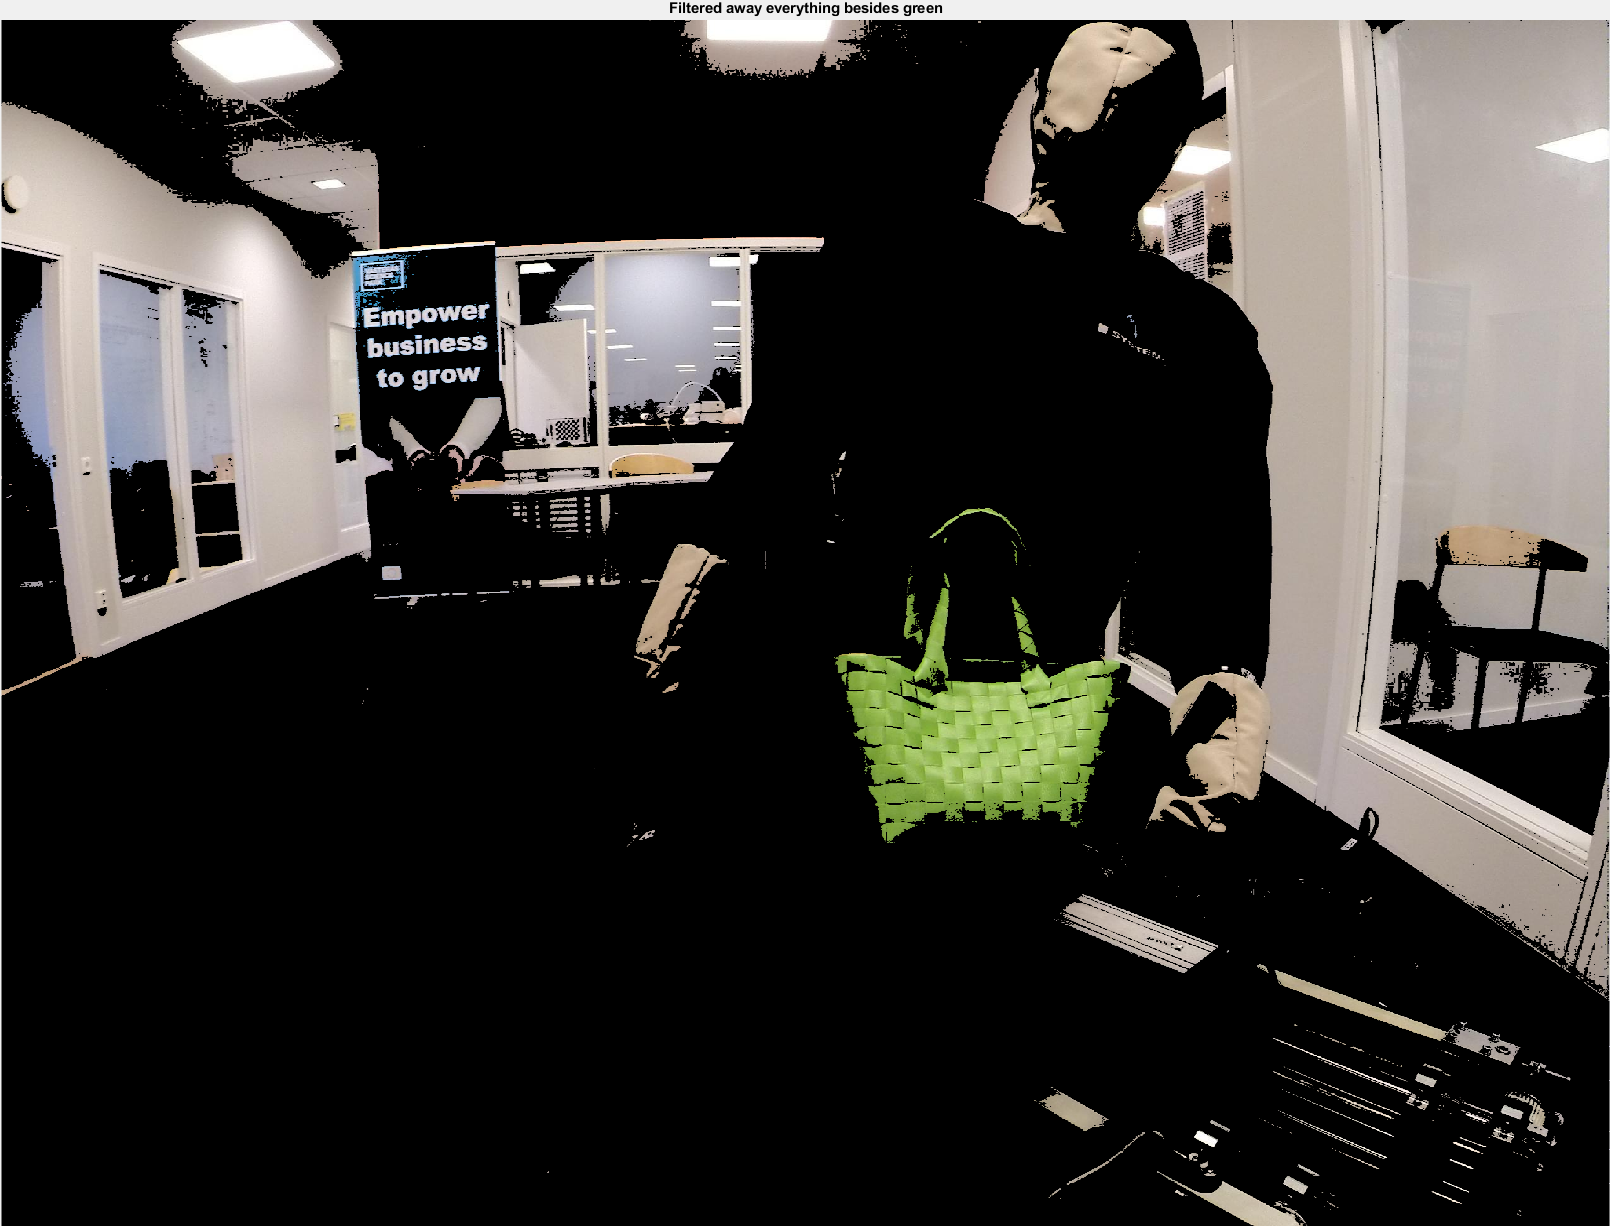
\includegraphics[width=\columnwidth]{images/green_filter.png}
    \caption{The created RGB green filter applied to bob image.}
    \label{fig:green_filter}
\end{figure}

\subsection{3.c.ii.}
The filter could be improved by not filtering based on RGB.

%-----------------------------------------------------------------------------

\subsection{3.d.i.}
The filter was created by tweaking the H, S and V parameters until a satisfactory result was obtained. H (hue) was the most important parameter, then S (saturation) and lastly V (value).

\subsection{3.d.ii.}
The color thresholder app filter which uses HSV is significantly better than the previous RGB filter, see Fig.\:\ref{fig:app_green_bag}.
\begin{figure}
    \centering
    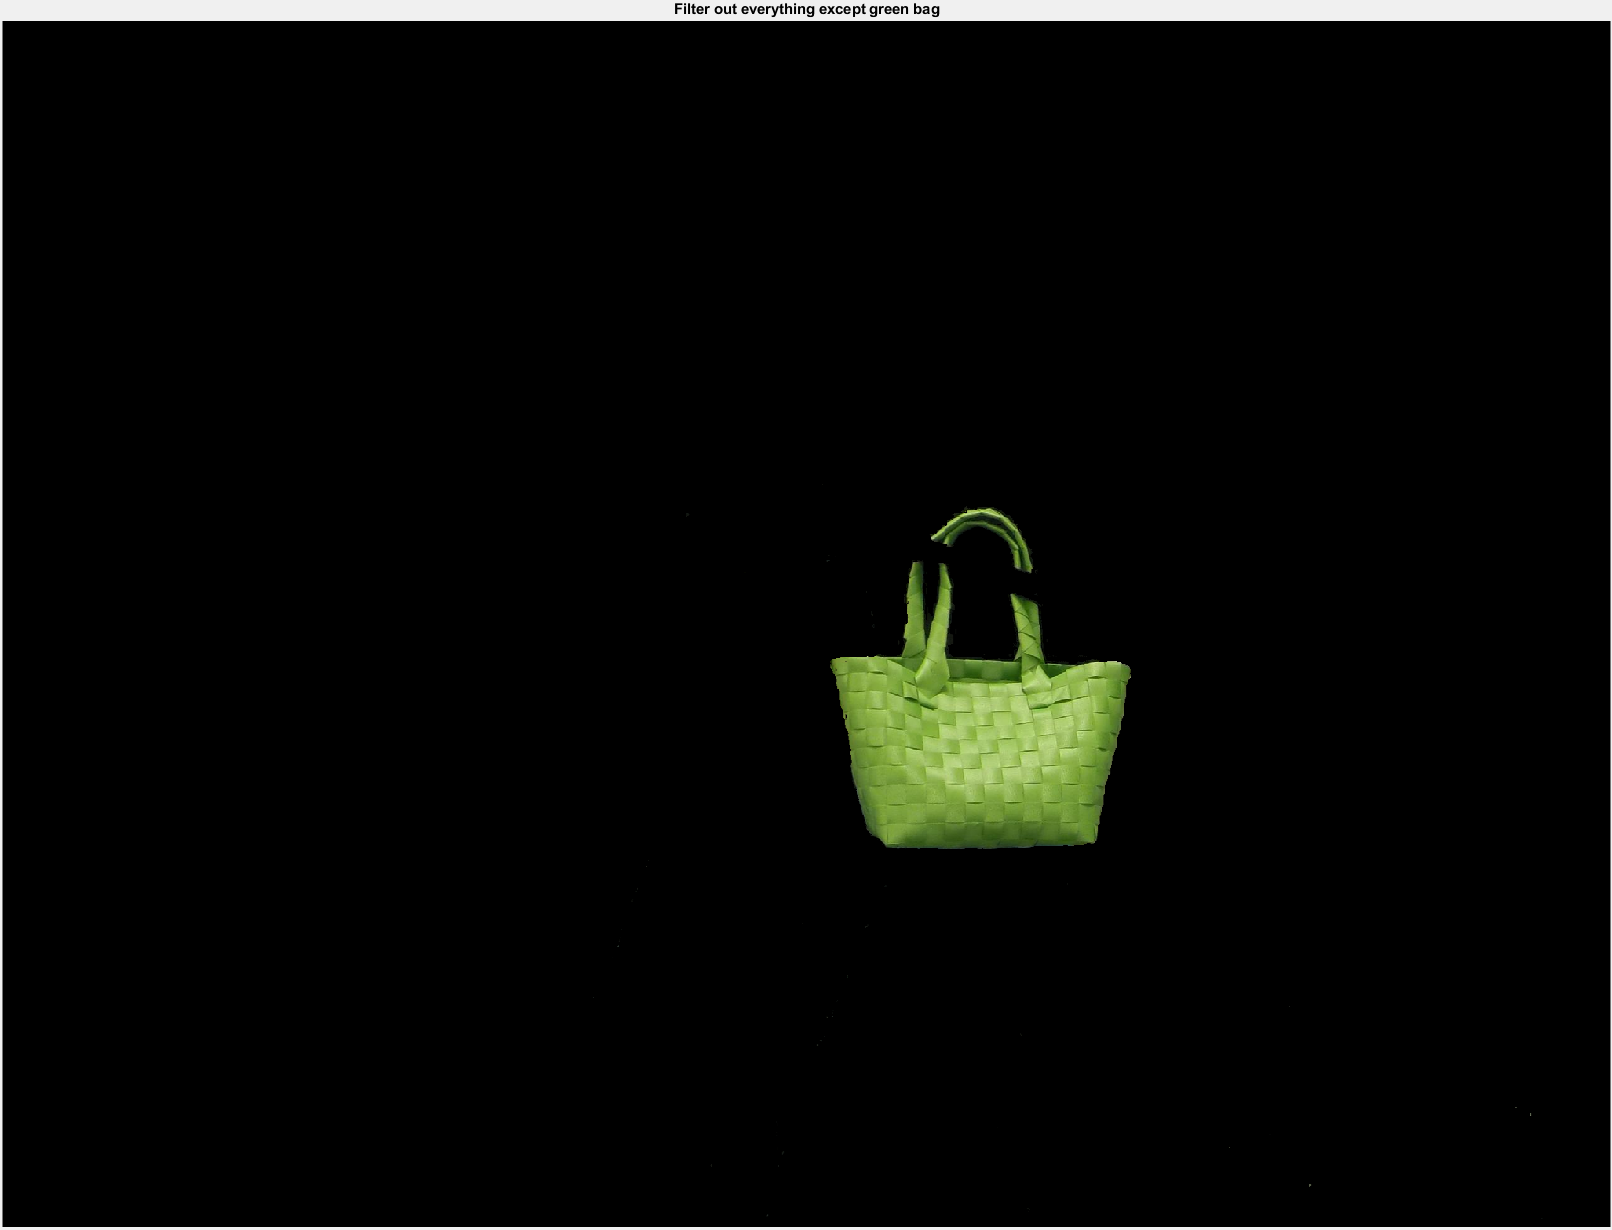
\includegraphics[width=\columnwidth]{images/app_green_bag.png}
    \caption{HSV green filter obtained using color thresholder app, applied to bob image.}
    \label{fig:app_green_bag}
\end{figure}

%-----------------------------------------------------------------------------
\subsection{3.e.i.}
To change the color of the bag, the mask obtained from the color thresholder app HSV filter (see previous subsection) was inverted, and then repeat the inverse of this mask for all R and G elements and then setting all elements which are 0 in the binary mask to $0$, thus only leaving blue.

\subsection{3.e.ii.}
The resulting color change of the bag to blue can be seen in Fig.\:\ref{fig:blue_bag}.
\begin{figure}
    \centering
    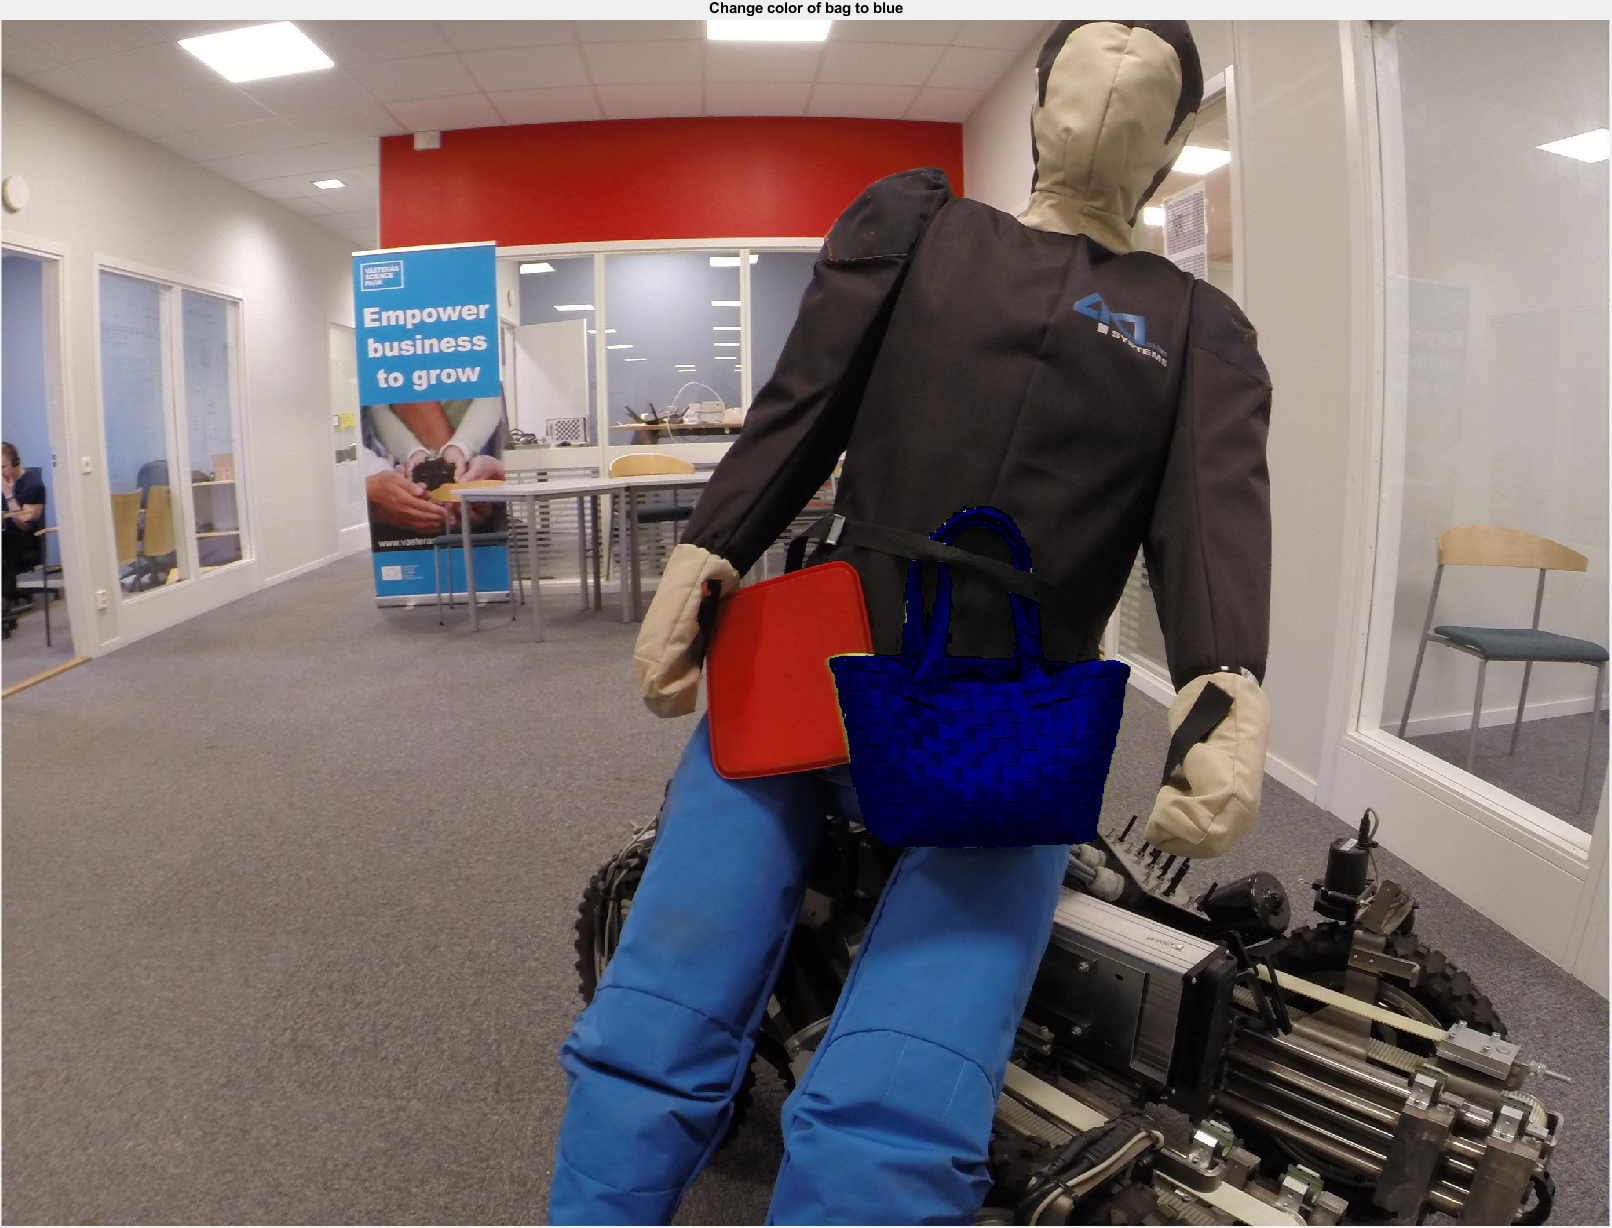
\includegraphics[width=\columnwidth]{images/blue_bag.png}
    \caption{Green bag in bob image changed to blue.}
    \label{fig:blue_bag}
\end{figure}

%-----------------------------------------------------------------------------

\subsection{4.d.i.}
They do provide the same results, see Fig.\:\ref{fig:associative}.
\begin{figure}
    \centering
    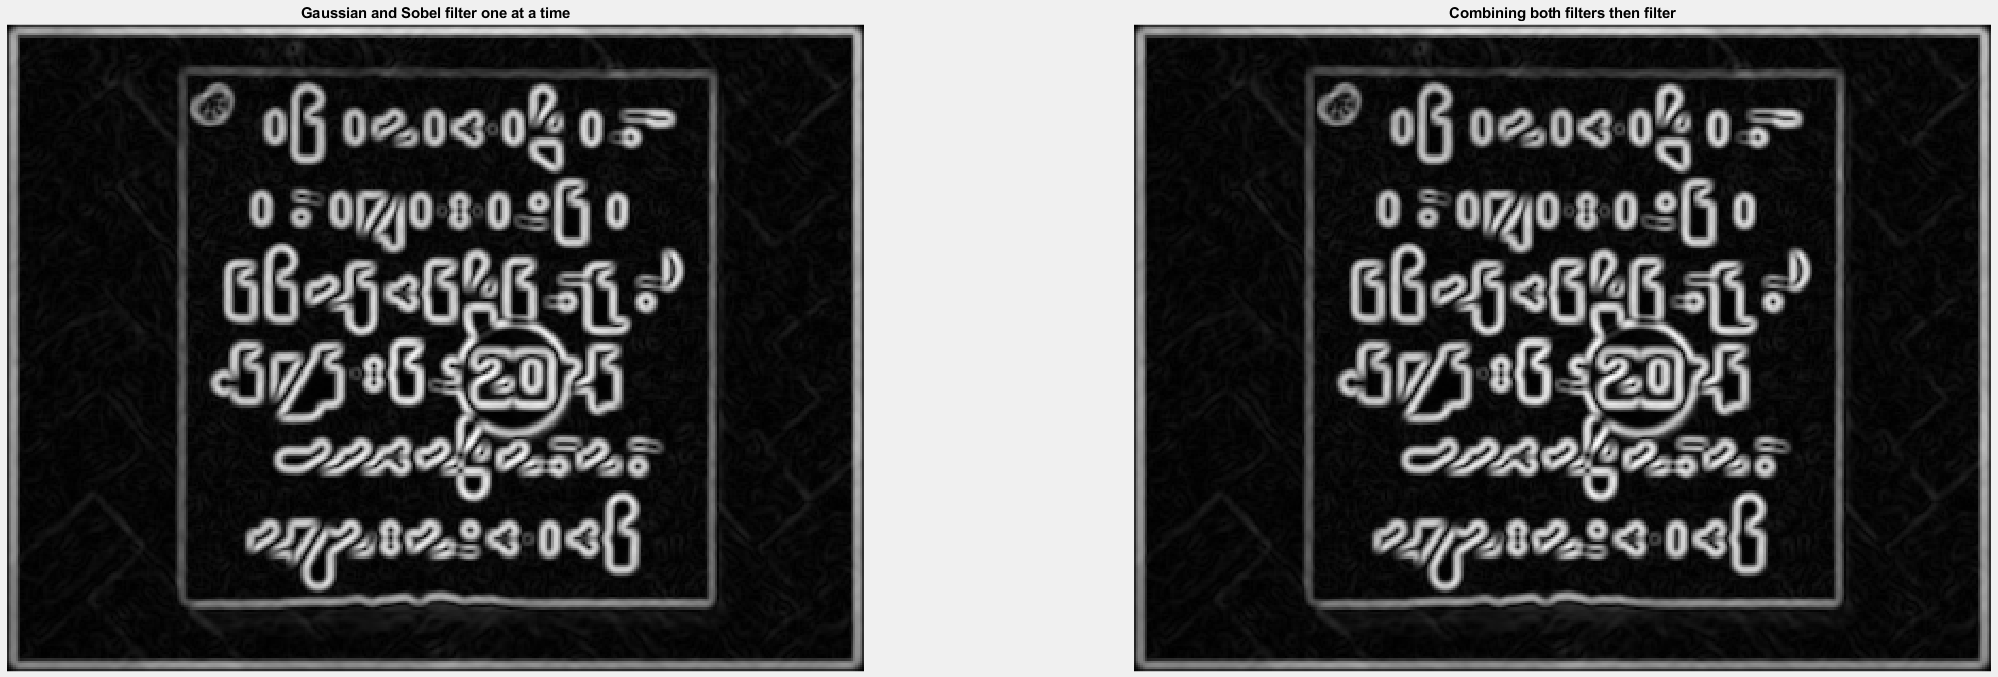
\includegraphics[width=\columnwidth]{images/associative.png}
    \caption{Comparison of convolution order on calendar image.}
    \label{fig:associative}
\end{figure}

\subsection{4.d.ii.}
Applying Gaussian and Sobel one at a time after each other was quicker, $0.42381\text{s}$ compared to $0.52601\text{s}$ for combining Gaussian and Sobel filters and then filtering. The reason for this is that combining Gaussian and Sobel requires one additional command since Gaussian needs to be applied to both the horizontal and the vertical parts of Sobel. But when they are applied one after another, then Gaussian can just be applied once to the image then filter Sobel vertical and horizontal after, rather than applying Gaussian to both vertical and horizontal Sobel.

%-----------------------------------------------------------------------------

\subsection{5.e.}
The result of the depth measurements can be seen in Table.\:\ref{tab:distance}.
\begin{table}
    \centering
    \begin{tabular}{c|c|c}
         Pen image                              & $1$           & $2$           \\ \hline
         Distance estimate (mm)                 & $390.0626$    & $428.9070$    \\
         Distance estimate undistorted (mm)     & $385.6962$    & $380.0242$
    \end{tabular}
    \caption{Estimated distance to pens using pinhole camera model.}
    \label{tab:distance}
\end{table}

From this, one can conclude that objects in distorted images can appear to be of a different size than they actually are, especially if they are close to the edges of the image. Undistorted images naturally reduces the error in this estimate. This leads to estimated distances to objects appearing to be further or closer than they actually are, when they are estimated based on a distorted image. This is once again also dependent on the location of the object in the image.

%-----------------------------------------------------------------------------
%\section{Results}
\label{section:results}
%\section{Discussion}
\label{section:disc}

%\section{Conclusion}
%\section*{Acknowledgment}

% Select the IEEEtran style
\bibliographystyle{IEEEtran}
% Include bibliography file
%\bibliography{references, refs}
\end{document}